\documentclass[aspectratio=169]{beamer}

\newcommand{\const}{\texttt{\bfseries const}}

\usepackage{fontspec}
\usepackage{listings}
\usepackage{tikz}

\usetikzlibrary{arrows}
\usetikzlibrary{calc}
\usetikzlibrary{decorations.pathreplacing}
\usetikzlibrary{fit}
\usetikzlibrary{matrix}
\usetikzlibrary{positioning}
\usetikzlibrary{tikzmark}
\usetikzmarklibrary{listings}

\definecolor{solarizedRed}{RGB}{220, 50, 47}
\definecolor{solarizedBlue}{RGB}{38, 139, 210}
\definecolor{solarizedGreen}{RGB}{133, 153, 0}
\definecolor{solarizedPurple}{RGB}{108, 113, 196}

\setbeamercolor{title}{fg=solarizedBlue}
\setbeamercolor{frametitle}{fg=solarizedBlue}
\setbeamercolor{structure}{fg=solarizedBlue}

\setbeamertemplate{navigation symbols}{}
\setbeamertemplate{headline}{}
\setbeamertemplate{footline}{}
\setbeamertemplate{itemize items}[circle]
%\setbeamertemplate{footline}[frame number]

\setbeamertemplate{footline}{
  \begin{tikzpicture}[remember picture,
                      overlay,
                      shift={(current page.south west)}]
    \node [black!50, inner sep=2mm, anchor=south east]
          at (current page.south east) {\large \insertframenumber};
  \end{tikzpicture}
}

\setsansfont{Overpass}[Scale=MatchLowercase]
\setmonofont{Overpass Mono}[Scale=MatchLowercase]

\lstset{
  basicstyle=\ttfamily\small,
  language=C++,
  escapeinside={(*@}{@*)},
  commentstyle={\color{black!45}},
}

\title{How C++ Developers Use Immutability Declarations: An Empirical Study}
\date{May 29, 2019}
\author{Jon Eyolfson}

\setbeamertemplate{title page}
{
  \begin{tikzpicture}[remember picture,
                      overlay,
                      shift={(current page.south west)}]
    \node (title) [inner sep=0, scale=2, align=left, text width=0.35\paperwidth]
          at (\paperwidth / 2, \paperheight * 2 / 3)
          {\bfseries
           \usebeamerfont{title}\usebeamercolor[fg]{title}\inserttitle};
    \node (author) [scale=1.5, align=left]
          at (\paperwidth / 3, \paperheight / 3)
          {{\bfseries \insertauthor}};

    \node [xshift=-4em, yshift=-4em]
          at (\paperwidth, \paperheight)
          {\includegraphics[scale=0.3]{../../image/acm-artifact-reusable.jpg}};
    \node [xshift=-4em, yshift=-11em]
          at (\paperwidth, \paperheight)
          {\includegraphics[scale=0.3]{../../image/acm-artifact-available.jpg}};

    \node (author2) [scale=1.5, align=left]
          at (\paperwidth * 2 / 3, \paperheight / 3)
          {Patrick Lam};
    \node [anchor=south west, inner sep=2mm] (cc-logo) at (0, 0)
          {\includegraphics[scale=0.2]{../../image/creativecommons-logo.eps}};
    \node [node distance=0, right=of cc-logo, xshift=-0.5em, yshift=-0.45em]
          {BY-SA 4.0};
    \node [anchor=south east, inner sep=2mm] at (\paperwidth, 0)
          {\texttt{1.0.0}};
    \node [anchor=south, inner sep=2mm] at ($(\paperwidth / 2, 0)$)
          {\insertdate};
    \node [node distance=0, below=of author]
          {\includegraphics[scale=0.1]{../../image/ucla-logo.eps}};
    \node [node distance=0, below=of author2, yshift=1.2em]
          {\includegraphics[scale=0.2]{../../image/uwaterloo-logo.eps}};
  \end{tikzpicture}
}

\begin{document}

  \begin{frame}[plain]
    \titlepage
  \end{frame}

  \setcounter{framenumber}{0}

  \begin{frame}[fragile]
    \frametitle{Immutability: Things Don't Change}

    Some languages allow developers to specify immutability using type
    qualifiers
    \begin{lstlisting}[xleftmargin=1cm]
class RNG {
public:
  int32_t getSeed(); // immutable
  int32_t getInt();  // possibly immutable?
};
    \end{lstlisting}

    As a developer you can have a mutable or immutable reference to \texttt{RNG}
    objects

    \begin{lstlisting}[xleftmargin=1cm]
/* immutable */ RNG rng;
rng.getInt(); // allowed?
    \end{lstlisting}

    \vspace{2em}

    \structure{Our question: how do developers use immutability?}
  \end{frame}

  \begin{frame}
    \frametitle{We Need to Pick a Language}

    C++ has immutability (using \texttt{const}) and much code available

    \vspace{1em}

    \hspace{1em} CppCoreGuideline: \structure{use \texttt{const} wherever
                 possible}

    \vspace{4em}

    Not clear that \texttt{const} is useful without a user study

    \vspace{1em}

    \hspace{1em} C++ \texttt{const} only aids developer understanding,
    it's not used for optimizations
  \end{frame}

  \begin{frame}[fragile]
    \frametitle{Add \texttt{const} to Methods Without Writes}

    \begin{columns}
      \begin{column}{0.4\textwidth}
        \begin{lstlisting}
class RNG {
public:
  int32_t getSeed() const {
    return seed;
  }
  int32_t getInt() {
    state = /* ... */;
    return state;
  }
private:
  int32_t seed;
  int32_t state;
};
        \end{lstlisting}
      \end{column}
      \begin{column}{0.5\textwidth}
        No writes to any fields, or writes through fields

        (deep concrete immutability)

        \vspace{1em}

        All developers can agree this is immutable

        \vspace{4em}

        \structure{No existing tools to assist in adding \texttt{const}}
      \end{column}
    \end{columns}
  \end{frame}

  \begin{frame}
    \frametitle{We Focus on Classes and Methods with Our \texttt{const} Checker Tool}

    How do developers use \texttt{const}?
    
    \vspace{1em}
    \hspace{1em} We manually inspect code with the help of our tool

    \vspace{4em}

    How well are developers using \texttt{const}?

    \vspace{1em}
    \hspace{1em} Our tool reports methods with deep concrete immutability
  \end{frame}

  \begin{frame}
    \frametitle{\texttt{const} Checker Analyzes Whole Codebases}

    We report classes that are defined within the codebase

    \vspace{2em}

    We use a lightweight static analysis to check writes to any
    fields

    \hspace{1em} or anything possibly reachable through fields

    \vspace{2em}

    Populate results into database, accessible through web interface
  \end{frame}

  \begin{frame}[fragile]
    \frametitle{Our Tool Reports \texttt{getSeed} as \texttt{const}}

    \begin{columns}
      \begin{column}{0.4\textwidth}
        \begin{lstlisting}
class RNG : public BaseRNG {
public:
  int32_t getSeed() {
    return seed;
  }
  int32_t getInt() {
    state = /* ... */;
    return state;
  }
private:
  int32_t state;
  int32_t seed;
};
        \end{lstlisting}
      \end{column}
      \begin{column}{0.5\textwidth}
        \texttt{getSeed} does not write \structure{(easily \texttt{const}-able)}

        \vspace{1em}

        \texttt{getInt} writes to a field

        \vspace{4em}

        This should be consistent with the base class
      \end{column}
    \end{columns}
  \end{frame}

  \begin{frame}[fragile]
    \frametitle{Our Analysis Uses Class Hierarchy to Remove Noise}
    \begin{columns}
      \begin{column}{0.4\textwidth}
        \begin{lstlisting}
class BaseRNG {
public:
  int32_t getSeed() {
    return 0;
  }
  int32_t getInt() {
    return 4;
  }
};
        \end{lstlisting}
      \end{column}
      \begin{column}{0.5\textwidth}
        This \texttt{getInt} should be \texttt{const}

        \hspace{1em} based only on method

        \vspace{2em}

        A subclass does however does mutate

        \hspace{1em} Our tool does not report as \texttt{const}
      \end{column}
    \end{columns}
  \end{frame}

  \begin{frame}
    \frametitle{We Ran Our Tool on 7 Large to Medium Projects}

    \begin{center}\begin{tabular}{l r r r}
                  & kLOC            & Classes & Methods \\
      \hline
      LLVM        & $\approx$ 3 200 &  10 518 &  55 229 \\
      OpenCV      &           1 167 &   2 220 &   6 624 \\
      Protobuf    &             625 &     407 &   1 813 \\
      fish        &             112 &     129 &     299 \\
      Mosh        &              14 &      74 &     302 \\
      Ninja       &              13 &      36 &     165 \\
      libsequence &              18 &      33 &     199 \\
    \end{tabular}\end{center}
  \end{frame}

  \begin{frame}
    \frametitle{We Study Non-Trivial Classes (>3 Methods)}

    Do developers write immutable classes? Classes that only mutate?

    \vspace{2em}

    \begin{center}\begin{tabular}{l r r}
                  & All \texttt{const} (\%) & Unannotated (\%) \\
      \hline
      LLVM        & 10 &  9 \\
      OpenCV      &  6 &  8 \\
      Protobuf    & 29 & 16 \\
      fish        &  0 & 21 \\
      Mosh        &  0 &  0 \\
      Ninja       &  0 & 12 \\
      libsequence & 50 &  2 \\
    \end{tabular}\end{center}
  \end{frame}

  \begin{frame}
    \frametitle{All-Mutating Classes are Rare}

    We estimated the true number by manual inspection (sampling for large
    projects)

    \vspace{2em}

    \begin{center}\begin{tabular}{l r r}
                  & Immutable (\%) & All-Mutating (\%) \\
      \hline
      LLVM        & 11 & 4 \\
      OpenCV      &  5 & 2 \\
      Protobuf    & 36 & 4 \\
      fish        &  0 & 7 \\
      Mosh        &  0 & 0 \\
      Ninja       &  0 & 0 \\
      libsequence & 50 & 0 \\
    \end{tabular}\end{center}
  \end{frame}

  \begin{frame}[fragile]
    \frametitle{OpenCV All-\texttt{const} Classes Were Not Immutable}

    \begin{lstlisting}
class _OutputArray {
public:
  void assign(/* ... */) const;
  void clear() const;
  void create(/* ... */) const;
  void release() const;
  bool needed() const;
  Mat & getMatRef(/* ... */) const;
};
    \end{lstlisting}
  \end{frame}

  \begin{frame}
    \frametitle{Most methods are \texttt{const}}

    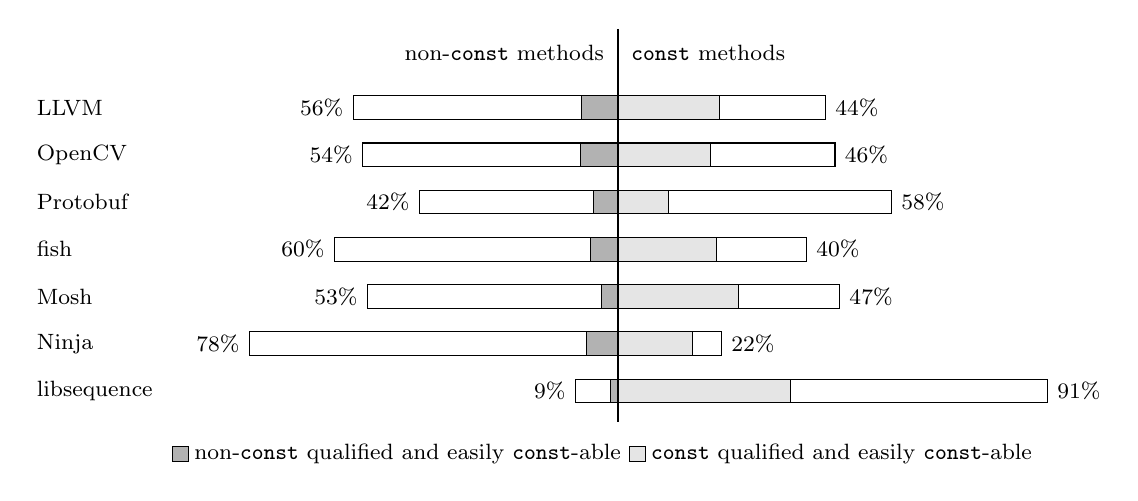
\begin{tikzpicture}
      \def\sideWidth{6}
    
      \def\projectAPercentageConst{44}
      \def\projectAPercentageNonConst{56}
      \def\projectAPercentageConstEasilyConstable{49.0}
      \def\projectAPercentageNonConstEasilyConstable{13.8}
      \pgfmathsetmacro\projectANonConstWidth{
        \sideWidth*\projectAPercentageNonConst/100
      }
      \pgfmathsetmacro\projectANonConstEasilyConstableWidth{
        \projectANonConstWidth*\projectAPercentageNonConstEasilyConstable/100
      }
      \pgfmathsetmacro\projectAConstWidth{
        \sideWidth*\projectAPercentageConst/100
      }
      \pgfmathsetmacro\projectAConstEasilyConstableWidth{
        \projectAConstWidth*\projectAPercentageConstEasilyConstable/100
      }
      \pgfmathsetmacro\projectAConstEasilyConstableHalfWidth{
        \projectAConstEasilyConstableWidth/2
      }
    
      \def\projectBPercentageConst{46}
      \def\projectBPercentageNonConst{54}
      \def\projectBPercentageConstEasilyConstable{42.6}
      \def\projectBPercentageNonConstEasilyConstable{14.5}
      \pgfmathsetmacro\projectBNonConstWidth{
        \sideWidth*\projectBPercentageNonConst/100
      }
      \pgfmathsetmacro\projectBNonConstEasilyConstableWidth{
        \projectBNonConstWidth*\projectBPercentageNonConstEasilyConstable/100
      }
      \pgfmathsetmacro\projectBConstWidth{
        \sideWidth*\projectBPercentageConst/100
      }
      \pgfmathsetmacro\projectBConstEasilyConstableWidth{
        \projectBConstWidth*\projectBPercentageConstEasilyConstable/100
      }
      \pgfmathsetmacro\projectBConstEasilyConstableHalfWidth{
        \projectBConstEasilyConstableWidth/2
      }
    
      \def\projectCPercentageConst{58}
      \def\projectCPercentageNonConst{42}
      \def\projectCPercentageConstEasilyConstable{18.6}
      \def\projectCPercentageNonConstEasilyConstable{12.1}
      \pgfmathsetmacro\projectCNonConstWidth{
        \sideWidth*\projectCPercentageNonConst/100
      }
      \pgfmathsetmacro\projectCNonConstEasilyConstableWidth{
        \projectCNonConstWidth*\projectCPercentageNonConstEasilyConstable/100
      }
      \pgfmathsetmacro\projectCConstWidth{
        \sideWidth*\projectCPercentageConst/100
      }
      \pgfmathsetmacro\projectCConstEasilyConstableWidth{
        \projectCConstWidth*\projectCPercentageConstEasilyConstable/100
      }
      \pgfmathsetmacro\projectCConstEasilyConstableHalfWidth{
        \projectCConstEasilyConstableWidth/2
      }
    
      \def\projectDPercentageConst{40}
      \def\projectDPercentageNonConst{60}
      \def\projectDPercentageConstEasilyConstable{52.1}
      \def\projectDPercentageNonConstEasilyConstable{9.6}
      \pgfmathsetmacro\projectDNonConstWidth{
        \sideWidth*\projectDPercentageNonConst/100
      }
      \pgfmathsetmacro\projectDNonConstEasilyConstableWidth{
        \projectDNonConstWidth*\projectDPercentageNonConstEasilyConstable/100
      }
      \pgfmathsetmacro\projectDConstWidth{
        \sideWidth*\projectDPercentageConst/100
      }
      \pgfmathsetmacro\projectDConstEasilyConstableWidth{
        \projectDConstWidth*\projectDPercentageConstEasilyConstable/100
      }
      \pgfmathsetmacro\projectDConstEasilyConstableHalfWidth{
        \projectDConstEasilyConstableWidth/2
      }
    
      \def\projectEPercentageConst{47}
      \def\projectEPercentageNonConst{53}
      \def\projectEPercentageConstEasilyConstable{54.5}
      \def\projectEPercentageNonConstEasilyConstable{6.3}
      \pgfmathsetmacro\projectENonConstWidth{
        \sideWidth*\projectEPercentageNonConst/100
      }
      \pgfmathsetmacro\projectENonConstEasilyConstableWidth{
        \projectENonConstWidth*\projectEPercentageNonConstEasilyConstable/100
      }
      \pgfmathsetmacro\projectEConstWidth{
        \sideWidth*\projectEPercentageConst/100
      }
      \pgfmathsetmacro\projectEConstEasilyConstableWidth{
        \projectEConstWidth*\projectEPercentageConstEasilyConstable/100
      }
      \pgfmathsetmacro\projectEConstEasilyConstableHalfWidth{
        \projectEConstEasilyConstableWidth/2
      }
    
      \def\projectFPercentageConst{22}
      \def\projectFPercentageNonConst{78}
      \def\projectFPercentageConstEasilyConstable{72.2}
      \def\projectFPercentageNonConstEasilyConstable{8.5}
      \pgfmathsetmacro\projectFNonConstWidth{
        \sideWidth*\projectFPercentageNonConst/100
      }
      \pgfmathsetmacro\projectFNonConstEasilyConstableWidth{
        \projectFNonConstWidth*\projectFPercentageNonConstEasilyConstable/100
      }
      \pgfmathsetmacro\projectFConstWidth{
        \sideWidth*\projectFPercentageConst/100
      }
      \pgfmathsetmacro\projectFConstEasilyConstableWidth{
        \projectFConstWidth*\projectFPercentageConstEasilyConstable/100
      }
      \pgfmathsetmacro\projectFConstEasilyConstableHalfWidth{
        \projectFConstEasilyConstableWidth/2
      }
    
      \def\projectGPercentageConst{91}
      \def\projectGPercentageNonConst{9}
      \def\projectGPercentageConstEasilyConstable{40.3}
      \def\projectGPercentageNonConstEasilyConstable{16.7}
      \pgfmathsetmacro\projectGNonConstWidth{
        \sideWidth*\projectGPercentageNonConst/100
      }
      \pgfmathsetmacro\projectGNonConstEasilyConstableWidth{
        \projectGNonConstWidth*\projectGPercentageNonConstEasilyConstable/100
      }
      \pgfmathsetmacro\projectGConstWidth{
        \sideWidth*\projectGPercentageConst/100
      }
      \pgfmathsetmacro\projectGConstEasilyConstableWidth{
        \projectGConstWidth*\projectGPercentageConstEasilyConstable/100
      }
      \pgfmathsetmacro\projectGConstEasilyConstableHalfWidth{
        \projectGConstEasilyConstableWidth/2
      }
      
      \node [anchor=west] at (-7.5, 0) {\footnotesize LLVM};
      \node [anchor=east] at (-\projectANonConstWidth, 0)
            {\footnotesize \projectAPercentageNonConst\%};
      \draw (-\projectANonConstWidth, 0.15) rectangle (0, -0.15);
      \draw [fill=black!30] (-\projectANonConstEasilyConstableWidth, 0.15)
            rectangle (0, -0.15);
      \draw [fill=black!10] (0, 0.15)
            rectangle (\projectAConstEasilyConstableWidth, -0.15);
      \draw (\projectAConstEasilyConstableWidth, 0.15)
            rectangle (\projectAConstWidth, -0.15);
      \node [anchor=west] at (\projectAConstWidth, 0)
            {\footnotesize \projectAPercentageConst\%};
    
      \node [anchor=west] at (-7.5, -0.6) {\footnotesize OpenCV};
      \node [anchor=east] at (-\projectBNonConstWidth, -0.6)
            {\footnotesize \projectBPercentageNonConst\%};
      \draw (-\projectBNonConstWidth, -0.45) rectangle (0, -0.75);
      \draw [fill=black!30] (-\projectBNonConstEasilyConstableWidth, -0.45)
            rectangle (0, -0.75);
      \draw [fill=black!10] (0, -0.45)
            rectangle (\projectBConstEasilyConstableWidth, -0.75);
      \draw (\projectBConstEasilyConstableWidth, -0.45)
            rectangle (\projectBConstWidth, -0.75);
      \node [anchor=west] at (\projectBConstWidth, -0.6)
            {\footnotesize \projectBPercentageConst\%};
    
      \node [anchor=west] at (-7.5, -1.2) {\footnotesize Protobuf};
      \node [anchor=east] at (-\projectCNonConstWidth, -1.2)
            {\footnotesize \projectCPercentageNonConst\%};
      \draw (-\projectCNonConstWidth, -1.05) rectangle (0, -1.35);
      \draw [fill=black!30] (-\projectCNonConstEasilyConstableWidth, -1.05)
            rectangle (0, -1.35);
      \draw [fill=black!10] (0, -1.05)
            rectangle (\projectCConstEasilyConstableWidth, -1.35);
      \draw (\projectCConstEasilyConstableWidth, -1.05)
            rectangle (\projectCConstWidth, -1.35);
      \node [anchor=west] at (\projectCConstWidth, -1.2)
            {\footnotesize \projectCPercentageConst\%};
    
      \node [anchor=west] at (-7.5, -1.8) {\footnotesize fish};
      \node [anchor=east] at (-\projectDNonConstWidth, -1.8)
            {\footnotesize \projectDPercentageNonConst\%};
      \draw (-\projectDNonConstWidth, -1.65) rectangle (0, -1.95);
      \draw [fill=black!30] (-\projectDNonConstEasilyConstableWidth, -1.65)
            rectangle (0, -1.95);
      \draw [fill=black!10] (0, -1.65)
            rectangle (\projectDConstEasilyConstableWidth, -1.95);
      \draw (\projectDConstEasilyConstableWidth, -1.65)
            rectangle (\projectDConstWidth, -1.95);
      \node [anchor=west] at (\projectDConstWidth, -1.8)
            {\footnotesize \projectDPercentageConst\%};
    
      \node [anchor=west] at (-7.5, -2.4) {\footnotesize Mosh};
      \node [anchor=east] at (-\projectENonConstWidth, -2.4)
            {\footnotesize \projectEPercentageNonConst\%};
      \draw (-\projectENonConstWidth, -2.25) rectangle (0, -2.55);
      \draw [fill=black!30] (-\projectENonConstEasilyConstableWidth, -2.25)
            rectangle (0, -2.55);
      \draw [fill=black!10] (0, -2.25)
            rectangle (\projectEConstEasilyConstableWidth, -2.55);
      \draw (\projectEConstEasilyConstableWidth, -2.25)
            rectangle (\projectEConstWidth, -2.55);
      \node [anchor=west] at (\projectEConstWidth, -2.4)
            {\footnotesize \projectEPercentageConst\%};
    
      \node [anchor=west] at (-7.5, -3) {\footnotesize Ninja};
      \node [anchor=east] at (-\projectFNonConstWidth, -3)
            {\footnotesize \projectFPercentageNonConst\%};
      \draw (-\projectFNonConstWidth, -2.85) rectangle (0, -3.15);
      \draw [fill=black!30] (-\projectFNonConstEasilyConstableWidth, -2.85)
            rectangle (0, -3.15);
      \draw [fill=black!10] (0, -2.85)
            rectangle (\projectFConstEasilyConstableWidth, -3.15);
      \draw (\projectFConstEasilyConstableWidth, -2.85)
            rectangle (\projectFConstWidth, -3.15);
      \node [anchor=west] at (\projectFConstWidth, -3)
            {\footnotesize \projectFPercentageConst\%};
    
      \node [anchor=west] at (-7.5, -3.6) {\footnotesize libsequence};
      \node [anchor=east] at (-\projectGNonConstWidth, -3.6)
            {\footnotesize \projectGPercentageNonConst\%};
      \draw (-\projectGNonConstWidth, -3.45) rectangle (0, -3.75);
      \draw [fill=black!30] (-\projectGNonConstEasilyConstableWidth, -3.45)
            rectangle (0, -3.75);
      \draw [fill=black!10] (0, -3.45)
            rectangle (\projectGConstEasilyConstableWidth, -3.75);
      \draw (\projectGConstEasilyConstableWidth, -3.45)
            rectangle (\projectGConstWidth, -3.75);
      \node [anchor=west] at (\projectGConstWidth, -3.6)
            {\footnotesize \projectGPercentageConst\%};
    
      \node [anchor=west] at (-5.5, -4.4)
            {\footnotesize non-\const{} qualified and easily \const{}-able};
      \draw [fill=black!30] (-5.45, -4.3) rectangle (-5.65, -4.5);
    
      \draw [fill=black!10] (0.15, -4.3) rectangle (0.35, -4.5);
      \node [anchor=west] at (0.3, -4.4)
            {\footnotesize \const{} qualified and easily \const{}-able};
    
      \node [anchor=east] at (-0.05, 0.7) {\footnotesize non-\const{} methods};
      \node [anchor=west] at (0.05, 0.7) {\footnotesize \const{} methods};
      \draw [thick] (0, 1) -- (0, -4);
    \end{tikzpicture}
  \end{frame}

  \begin{frame}
    \frametitle{Slighty Over Half of Methods are \texttt{const}}

    Our manual inspection showed all of the methods we reported were
    \texttt{const}-able

    \vspace{2em}

    Overall we estimated the number of truly \texttt{const} methods (\%) as:

    \vspace{1em}
    
    \begin{center}\begin{tabular}{l r}
      LLVM         & 52\\
      OpenCV       & 53\\
      Protobuf     & 63 \\
      fish shell   & 46 \\
      Mosh         & 51 \\
      Ninja        & 28 \\
      libsequence  & 93 \\
    \end{tabular}\end{center}
  \end{frame}

  \begin{frame}
    \frametitle{Developers Do Use Immutability, Extensively}

    Immutable classes represent around 12\% of classes

    \hspace{1em} All-mutating classes are rare (4\%)

    \vspace{2em}

    Most classes contain a mixture of \texttt{const} and mutable methods

    \hspace{1em} Overall, half these methods are \texttt{const} (52\% median)
  \end{frame}

  \begin{frame}
    \frametitle{Our Tool is Freely Available!}

    Available and Reusable from Artifact Evaluation

    \vspace{2em}

    \url{https://github.com/eyolfson/const-checker-artifact}

    \vspace{2em}

    It's simple to add more projects
  \end{frame}

  \begin{frame}
    \frametitle{Developers Want Immutability}

    Overall 12\% of classes were immutable

    \hspace{1em} in 3 projects it was 0\%

    \vspace{1em}

    The remaining 84\% of classes contain a mixture

    \vspace{1em}

    \structure{Languages need more than immutable classes}

    \vspace{4em}

    Developers do label the majority of \texttt{const} methods

    \hspace{1em} Our tool showed them missing 12\% of mutable methods (at
                 minimum)

    \vspace{1em}

    \structure{Developers need better tools}
  \end{frame}

\end{document}
